\documentclass[12pt,twoside, a4paper, twocolumn]{article}
\usepackage[utf8]{inputenc}
\usepackage[brazil]{babel}
\usepackage[margin = 0.5in]{geometry}
\usepackage{amsmath}
\usepackage{amsthm}
\usepackage{amssymb}
\usepackage{amsthm}
\usepackage{setspace}
\usepackage[americanvoltages,fulldiodes,siunitx]{circuitikz}
\usepackage{lipsum}
\usepackage{pgfplots}
\usepackage{ifthen}
\usepackage{adjustbox}
\usepackage[section]{placeins}
\usepackage{hyperref}
\usepackage{graphicx}
 
 
\graphicspath{ {./images/} }
\pgfplotsset{compat=newest}
 
 
 
%  #1 color - optional #2 x_0 #3 y_0 #4 x_f #5 y_f #6 name - optional  #7 true if adding lines to axis
 
\newcommand{\drawvector} [9] [color=cyan] {
   \draw[line width=1.5pt,#1,-stealth](axis cs: #2, #3)--(axis cs: #4, #5) node[anchor=south west]{$#6$};
 
  
 
\ifthenelse{\equal{#7}{true}}{
   \draw[line width=1pt,#1, dashed](axis cs: #4, #5)--(axis cs: #4, 0) node[anchor= north west]{$#8$};
   \draw[line width=1pt,#1, dashed](axis cs: #4, #5)--(axis cs: 0, #5) node[anchor=south east]{$#9$};
   }
   {}
}
 
\newcommand\deriv[2]{\frac{\mathrm d #1}{\mathrm d #2}}
 
 
\title{Primeiro Relatório de Física Experimental 2}
\author{Henrique da Silva \\ hpsilva@proton.me}
\date{\today}
\pgfplotsset{width = 10cm, compat = 1.9}
 
 
\begin{document}
\maketitle
\pagenumbering{gobble}
\newpage
%pagenumbering{roman}
\tableofcontents
\newpage

\section{Introdução}

\paragraph*{Neste relatório, vamos fazer medições de resistência, voltagem, e corrente de um circuito de corrente contínua com três tipos de elementos resistivos, e vamos averiguar seu comportamento em cada caso.}



\paragraph*{Todos arquivos utilizados para criar este relatório, e o relatório em si estão em:  \url{https://github.com/Shapis/ufpe_ee/tree/main/4th semester/fisica experimental 2}}


\section{Circuito simples}

\begin{center}
    \begin{circuitikz}
        \draw
        (0,0) to[battery1,  invert] (0,2) % l=5<\milli\volt>
        to[rmeter, t=A] (4,2) -- (4,0) to [resistor] (0,0)
        (3,0) -- (3,-1.5)  to[rmeter, t=V] (1,-1.5) - - (1,0)
        ;
        \draw (0,-0.05)
        node[rground]{};
    \end{circuitikz}
\end{center}

\subparagraph*{Neste circuito vamos ter uma corrente saindo de uma fonte de tensão, e entrando num amperímetro, do amperímetro passará por um resistor e um voltímetro em série, e daí voltará para a fonte.}
\subsection{Tabela de dados}
\begin{center}
    \begin{tabular}{ |cc| }
        \hline
        Tensão (V)        & Corrente (mA)     \\
        $0.44$ $\pm0.05$  & $20$ $\pm10$      \\
        $1.03$ $\pm0.05$  & $40$     $\pm10$  \\
        $1.57$ $\pm0.05$  & $60$     $\pm10$  \\
        $2.06$ $\pm0.05$  & $80$      $\pm10$ \\
        $2.68$ $\pm0.05$  & $100$     $\pm10$ \\
        $3.48$ $\pm0.05$  & $120$     $\pm10$ \\
        $3.67$  $\pm0.05$ & $140$     $\pm10$ \\
        $4.16$ $\pm0.05$  & $160$     $\pm10$ \\
        $4.86$ $\pm0.05$  & $180$     $\pm10$ \\
        $5.47$ $\pm0.05$  & $200$     $\pm10$ \\

        \hline
    \end{tabular}
\end{center}



\subsection{Gráfico de corrente por Tensão }
\subparagraph*{No gráfico, devemos esperar que a inclinação da reta será dado por $\frac{1}{R}$ se o comportamento for Ôhmico, já que: }

\begin{equation}
    \begin{aligned}
        V & = I R           \\
        I & = \frac{V}{R}   \\
        I & = \frac{1}{R} V \\
    \end{aligned}
\end{equation}
\begin{adjustbox}{scale=0.70}
    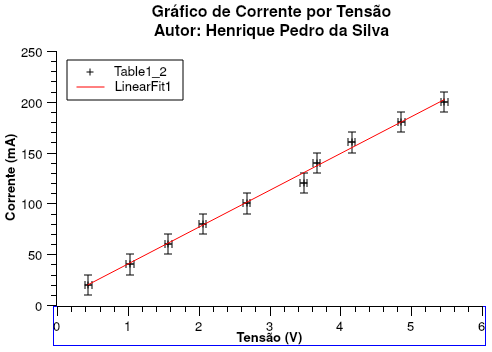
\includegraphics{Graph1.png}
\end{adjustbox}

\subparagraph*{Fazendo um fit linear no SciDAVis consigo que o valor da inclinação $\frac{1}{R}$ eh $0.03624$  que implica pela relação conseguida em (1) que $ R_{total} = 28 \pm 1 \varOmega$. E isso nos confirma que o sistema se comporta de maneira Ôhmica.}

\subparagraph*{Cálculo da incerteza abaixo:}

\begin{equation}
    \begin{aligned}
        \deriv{R}{V}      & = \frac{1}{V}                                          \\
        \deriv{R}{I}      & = - \frac{V}{I^2}                                      \\
        \varDelta_{total} & = sqrt{\left( \deriv{R}{I}^2 + \deriv{R}{V}^2 \right)} \\
        \varDelta_{total} & = 1                                                    \\
    \end{aligned}
\end{equation}



\subsection{Averiguando resistência do Amperímetro}
\subparagraph*{É importante notar que a resistência que consegui no item (2.1.3)  não é a resistência do resistor, mas sim a resistência do sistema inteiro. Que é:}

\begin{equation*}
    R_{resistor} + R_{amperimetro} + R_{conexoes} + R_{fios}
\end{equation*}

\subparagraph*{Para simplificar os cálculos dos itens a seguir vou considerar que toda resistência do sistema está no resistor e no amperímetro apenas.}

\subparagraph*{Com o amperímetro medimos $2.65V$ e sem ele medimos $2.5V$}

\subparagraph*{Já que os elementos estão em série podemos dizer que:}

\begin{equation}
    \begin{aligned}
        V_1 & = I (R_{resistor} + R_{amperimetro}) \\
        V_2 & = I R_{resistor}                     \\
    \end{aligned}
\end{equation}

\subparagraph*{E já calculamos o valor da resistência total no item anterior e sua devida incerteza.}

\subparagraph*{Logo só o que preciso é calcular o $R_{resistor}$ a partir do $\frac{V_2}{I}$ e o subtrair da resistência total do sistema que já havia sido calculada.}

\begin{equation}
    \frac{2.5}{0.1} = 25 \varOmega
\end{equation}

\subparagraph*{Calculando a incerteza da mesma maneira de (2), temos que ela será $1 \varOmega$}

\subparagraph*{Subtraindo o valor da resistência total pelo valor da resistência do resistor finalmente temos que:}

\begin{equation}
    R_{amperimetro} = 3 \pm 2 \varOmega
\end{equation}

\subparagraph*{Uma maneira alternativa de obter isso seria:}

\begin{equation}
    V_{ca} = R_{resistor} * \left( \frac{V_0}{R_{amp} + R_{resistor}} \right)
\end{equation}

\subparagraph*{Meu problema com isso, é que a priori eu não tenho a resistência do resistor. Apenas tenho a do sistema total. Então eu teria que assumir que ela eh 27 baseado em conhecimento que não foi obtido através dos experimentos. Logo optei pela maneira acima que descrevi.}

\subsection{Averiguando resistência do voltímetro}

\subparagraph*{Com ou sem o voltímetros a corrente se manteve firme em $190mA$. }

\subparagraph*{O que indica que a resistência do voltímetros é alta o suficiente para não ser mensurável.}

\section{Circuito com resistor e lâmpada}

\begin{center}
    \begin{circuitikz}
        \draw
        (0,0) to[battery1,  invert] (0,2) % l=5<\milli\volt>
        to[resistor] (2,2) to[rmeter, t=L] (4,2) to [rmeter, t=A] (4,0) -- (0,0)

        ;
        \draw (0,-0.05)


        node[rground]{};

    \end{circuitikz}
\end{center}

\subparagraph*{Neste circuito vamos ter uma corrente saindo de uma fonte de tensão, e entrando num amperímetro, do amperímetro passará por um resistor, daí para uma lâmpada, e daí voltará para a fonte.}

\subparagraph*{Faremos medições diversas com um voltímetro em vários pontos do circuito.}
\subsection{Tabela de dados}
\begin{center}
    \begin{tabular}{ |ccc| }
        \hline
        Corrente (mA) & Tensão R (V)     & Tensão L (V)     \\
        $10$ $\pm10$  & $0.33$ $\pm0.05$ & $0.06$ $\pm0.05$ \\
        $20$ $\pm10$  & $0.46$ $\pm0.05$ & $0.11$ $\pm0.05$ \\
        $30$ $\pm10$  & $0.77$ $\pm0.05$ & $0.19$ $\pm0.05$ \\
        $40$ $\pm10$  & $0.97$ $\pm0.05$ & $0.40$ $\pm0.05$ \\
        $50$ $\pm10$  & $1.32$ $\pm0.05$ & $0.47$ $\pm0.05$ \\
        $60$ $\pm10$  & $1.61$ $\pm0.05$ & $0.53$ $\pm0.05$ \\
        $70$ $\pm10$  & $1.93$ $\pm0.05$ & $0.70$ $\pm0.05$ \\
        $80$ $\pm10$  & $2.20$ $\pm0.05$ & $0.76$ $\pm0.05$ \\
        $90$ $\pm10$  & $2.35$ $\pm0.05$ & $0.83$ $\pm0.05$ \\
        $100$ $\pm10$ & $2.53$ $\pm0.05$ & $1.01$ $\pm0.05$ \\
        $110$ $\pm10$ & $2.86$ $\pm0.05$ & $1.18$ $\pm0.05$ \\
        $120$ $\pm10$ & $3.12$ $\pm0.05$ & $1.42$ $\pm0.05$ \\
        $130$ $\pm10$ & $3.39$ $\pm0.05$ & $1.64$ $\pm0.05$ \\
        $140$ $\pm10$ & $3.67$ $\pm0.05$ & $2.00$ $\pm0.05$ \\
        $150$ $\pm10$ & $4.00$ $\pm0.05$ & $2.20$ $\pm0.05$ \\
        $160$ $\pm10$ & $4.27$ $\pm0.05$ & $2.45$ $\pm0.05$ \\
        $170$ $\pm10$ & $4.54$ $\pm0.05$ & $2.66$ $\pm0.05$ \\
        $180$ $\pm10$ & $4.77$ $\pm0.05$ & $2.89$ $\pm0.05$ \\
        $190$ $\pm10$ & $4.96$ $\pm0.05$ & $3.04$ $\pm0.05$ \\
        $200$ $\pm10$ & $5.28$ $\pm0.05$ & $3.36$ $\pm0.05$ \\


        \hline
    \end{tabular}
\end{center}

\subsection{Comportamento da Lampada}

\begin{equation*}
    \begin{aligned}
        I = 20mA  & \rightarrow 5.5 \varOmega  \\
        I = 100mA & \rightarrow 10.1\varOmega  \\
        I = 200mA & \rightarrow 16.8 \varOmega \\
    \end{aligned}
\end{equation*}

\subparagraph*{Logo detectamos um comportamento não ômico. Já que a resistência sobe com a corrente.}

\subparagraph*{O que é esperado. Já que o que esperávamos é que a resistência subisse à medida que a temperatura da lâmpada subisse.}

\subsection{Gráficos I - V para resistor e lâmpada}

\begin{adjustbox}{scale=0.70}
    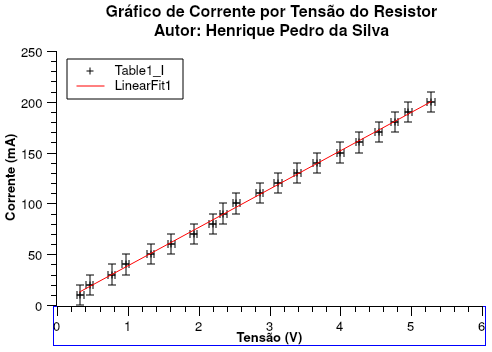
\includegraphics{Graph2.png}
\end{adjustbox}

\begin{adjustbox}{scale=0.70}
    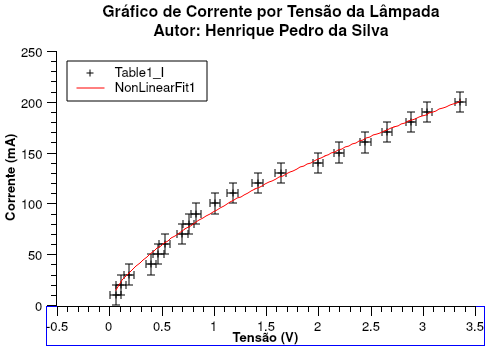
\includegraphics{Graph3.png}
\end{adjustbox}

\begin{adjustbox}{scale=0.70}
    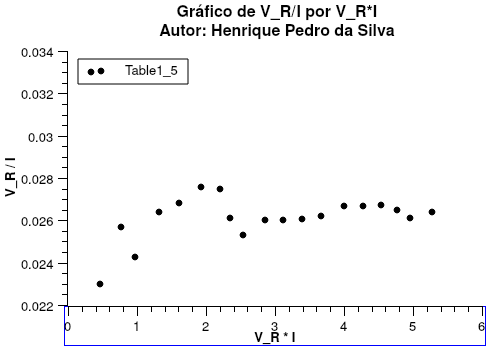
\includegraphics{Graph4.png}
\end{adjustbox}

\begin{adjustbox}{scale=0.70}
    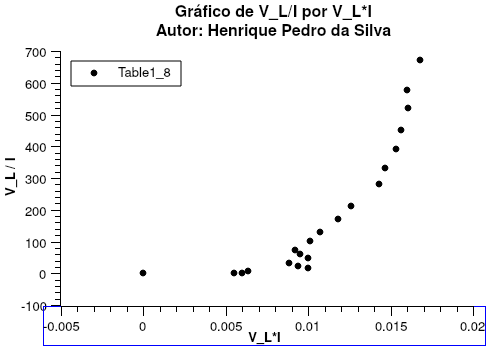
\includegraphics{Graph5.png}
\end{adjustbox}

\subsection{Conclusões}

\subparagraph*{Podemos observar que o resistor continua com um comportamento Ohmico. Porem a lampada nao. Nesta a resistência aumenta com a corrente.}

\section{Circuito com resistor e diodo}

\begin{center}
    \begin{circuitikz}
        \draw
        (0,0) to[battery1,  invert] (0,2) % l=5<\milli\volt>
        to[resistor] (2,2) to[diode] (4,2) to [rmeter, t=A] (4,0) -- (0,0)

        ;
        \draw (0,-0.05)


        node[rground]{};

    \end{circuitikz}
\end{center}

\subsection{Sentido do diodo}

\subparagraph*{O diodo só permite passagem de corrente de $10mA$ em um sentido. No sentido oposto não foi detectado corrente alguma.}

\subparagraph*{Isso é devido ao diodo ser feito por dois semicondutores em uma junção PN. Que só permite passagem de corrente em um sentido.}

\subparagraph*{Algo interessante que foi notado é que mesmo sem passagem de corrente é detectável uma diferença de potencial dos terminais do diodo. Isso acontece devido a polarização que ocorre nele.}

\subsection{Tabela de dados}
\begin{center}
    \begin{tabular}{ |ccc| }
        \hline
        Corrente (mA) & Tensão R (V)     & Tensão D (V)     \\
        $0$ $\pm10$   & $0$ $\pm0.05$    & $0.10$ $\pm0.05$ \\
        $0$ $\pm10$   & $0$ $\pm0.05$    & $0.20$ $\pm0.05$ \\
        $0$ $\pm10$   & $0$ $\pm0.05$    & $0.30$ $\pm0.05$ \\
        $0$ $\pm10$   & $0$ $\pm0.05$    & $0.40$ $\pm0.05$ \\
        $0$ $\pm10$   & $0$ $\pm0.05$    & $0.50$ $\pm0.05$ \\
        $0$ $\pm10$   & $0$ $\pm0.05$    & $0.60$ $\pm0.05$ \\
        $10$ $\pm10$  & $0.40$ $\pm0.05$ & $0.70$ $\pm0.05$ \\
        $50$ $\pm10$  & $1.27$ $\pm0.05$ & $0.74$ $\pm0.05$ \\
        $90$ $\pm10$  & $2.40$ $\pm0.05$ & $0.77$ $\pm0.05$ \\
        $130$ $\pm10$ & $3.44$ $\pm0.05$ & $0.78$ $\pm0.05$ \\
        $170$ $\pm10$ & $4.57$ $\pm0.05$ & $0.79$ $\pm0.05$ \\
        $200$ $\pm10$ & $5.26$ $\pm0.05$ & $0.80$ $\pm0.05$ \\



        \hline
    \end{tabular}
\end{center}


\subsection{Gráficos I - V para resistor e diodo}

\begin{adjustbox}{scale=0.70}
    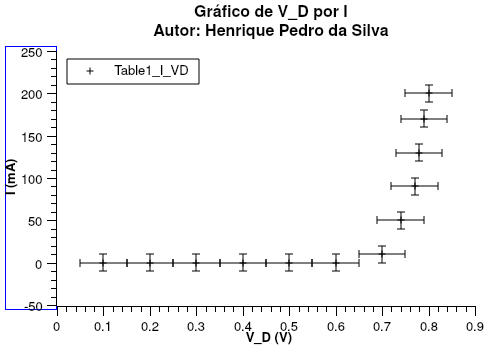
\includegraphics{Graph6.png}
\end{adjustbox}

\subparagraph*{As características obtidas foram similares às de um diodo ideal.}

\subparagraph*{O esperado é que mesmo antes da resistência do diodo ser vencida pela diferença de potencial, ainda passasse alguma corrente, mesmo que mínima. }

\subparagraph*{Porém esta foi tão baixa que foi indetectável.}


\subsection{Conclusões}

\subparagraph*{Se repara que é necessária certa tensão no diodo para permitir passagem de corrente.}

\subparagraph*{A partir de certa tensão o diodo permite passagem de corrente.}

\subparagraph*{O comportamento de um diodo ideal seria não passar corrente alguma até haver uma diferença de potencial suficiente para permitir a passagem.}

\subparagraph*{No nosso diodo nao ideal, logo sabemos que ele permitirá passagem de alguma corrente, porém esta foi baixa o suficiente para não ser detectável}

\subparagraph*{E por fim, este não apresenta comportamento Ôhmico. Ja que após permitir passagem de corrente, a diferença de potencial dos seus terminais se manteve quase constante.}



\end{document}